\section{Experiments}
\label{section:experiments}

In this section, the proposed model is applied to two benchmark synthetic datasets (Pinwheel
and Two-circles) and one real-world dataset (MNIST). On one of the synthetic
datasets, one shortcoming of the model is brought to attention, but is overcome
in a semi-supervised setting. On the real-world dataset, the model's clustering
capabilities are evaluted, as well as its capacity to model complex distributions.

A technique inspired in the work of \textcite{mixae} was employed to improve training
speed and quality of results. This consists in dividing the inputs of the softmax layer in
the variational posterior by a \q{temperature} value, $T$, which follows
an exponential decay schedule during training. Intuitively, this makes the
variational posterior \q{more certain} as training proceeds, while allowing all
components to be generally exposed to the whole data, during the initial epochs.
This discourages components from being \q{subtrained} during the initial epochs
and, subsequently, from being prematurely discarded by the variational posterior.

\subsection{Toy datasets}
\subsubsection{Pinwheel dataset}

This dataset is constituted by five non-linear \q{wings}. See Figure \ref{fig:pinwheel}
for the results of running the model on this dataset. As expected, the variational
posterior has learned to partition the space so as to attribute each \q{wing} to
a component of the mixture. This partitioning is imperfect in regions of space
that have low probability for every component.

\begin{figure}[!htb]
  \begin{subfigmatrix}{2}
    \subfigure[]{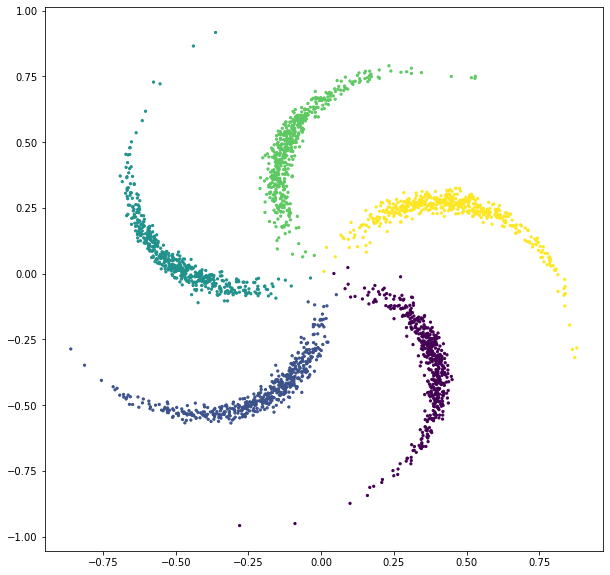
\includegraphics[width=0.49\linewidth]{figures/original_pinwheel.png}}
    \subfigure[]{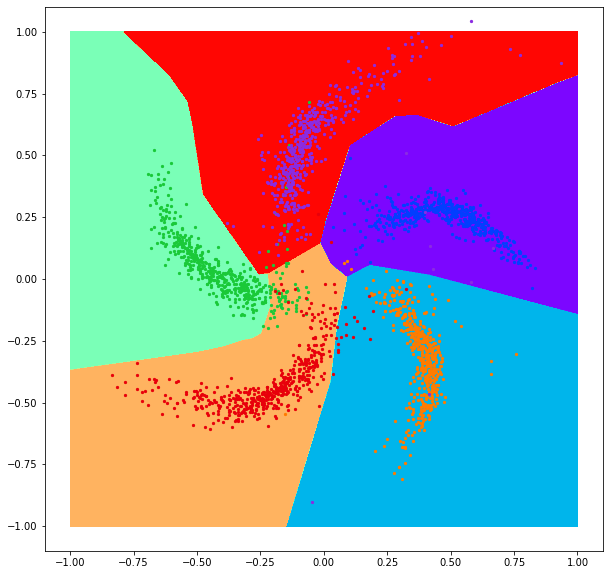
\includegraphics[width=0.49\linewidth]{figures/trained_pinwheel.png}}
  \end{subfigmatrix}
    \caption{(a) Original dataset. (b) Samples from the learned model. Each
dot is colored according to the component it was sampled from. The background
colors denote the regions where each component has maximum probability assigned
by the variational posterior. (Note that the background colors were chosen
so as to not match the dot colors, otherwise the dots would not be visible)}
  \label{fig:pinwheel}
\end{figure}

This experiment consisted of training on 2560 data points (512 per class) using
the Adam optimizer, with a learning rate of 0.001, a
mini-batch size of 512, during 400 epochs. The variational posterior was parameterized
by a multi-layer perceptron, with 1 hidden layer of dimension 3, and a
softmax output. Each component of the mixture was a RealNVP with 8 blocks, each
block with multi-layer perceptrons, with 1 hidden layer of dimension 8 as the
$s(.)$ and $t(.)$ functions of the affine coupling layers.

\subsubsection{Two-circles dataset}
This dataset consists of two concentric circles. The experiment on this dataset,
shown on Figure \ref{fig:twocircles}, makes evident one shortcoming of this
model: the way in which the variational posterior partitions the space is
not necessarily guided by the intrisic structure in the data. In the case of
the two-circles dataset, it was found that the most common space partitioning
induced by the model consisted simply of splitting into two half-spaces. However, in
a semi-supervised setting, this behaviour can be corrected and the model
successfully learns to separate the two circles, as shown in Figure
\ref{fig:twocircles-semisup}. In this setting, the model was pretrained on
the labeled instances for some epochs and then trained with the normal procedure.
In the semi-supervised setting, the model has the chance to refine both the
variational posterior and each of the components, thus making better use of
the unlabeled data in the unsupervised phase of the training. As is clearly
visible in Figure \ref{fig:twocircles-semisup}, the model struggles with
learning full, closed, circles; this is because it is unable to \q{pierce a hole}
in the base distribution, due to the nature of the transformations that are
applicable. Thus, to model a circle, the model has to learn to stretch the blob
formed by the base distribution, and \q{bend it over itself}. This difficulty
is also what keeps the model from learning a structurally interesting solution
in the fully unsupervised case: it is easier to learn to distort space so as to
learn a multimodal distribution that models half of the two circles. Moreover,
the points in diametrically opposed regions of the same circle are more dissimilar
(in the geometrical sense) than points in the same region of the two circles.
Therefore, when completely uninformed by labels, the variational posterior's
layers will tend to have similar activations for points in the latter case, and
thus tend to place them in the same class.

The unsupervised learning experiment consisted of training on 1024 datapoints,
512 per class; using the Adam optimizer, with a learning rate
of 0.001, a mini-batch size of 128, during 500 epochs.
The semi-supervised learning experiment consisted of training on 1024 unlabeled
datapoints, 512 per class and 64 labeled data points, 32 per class. The model
was first pretrained during 300 epochs solely on the 32 labeled data points, using
the labels to selectively optimize each component of the mixture, as well as
to optimize the variational posterior by minimizing a binary cross-entropy loss.
After pretraining, the model was trained by interweaving supervised epochs - like
in pretraining - with unsupervised epochs. Optimization was carried out using the
Adam optimizer, with a learning rate of 0.001, a mini-batch size of 128, during 500 epochs.
For both the unsupervised and the semi-supervised experiments, the neural network
used to parameterize the variational posterior was a multi-layer perceptron, with
2 hidden layers of dimension 16, and with a softmax output. Each component of the
mixture was a RealNVP with 10 blocks, each block with multi-layer perceptrons,
with 1 hidden layer of dimension 8, as the $s(.)$ and $t(.)$ functions of the
affine coupling layers.

\begin{figure}[!htb]
  \begin{subfigmatrix}{2}
    \subfigure[]{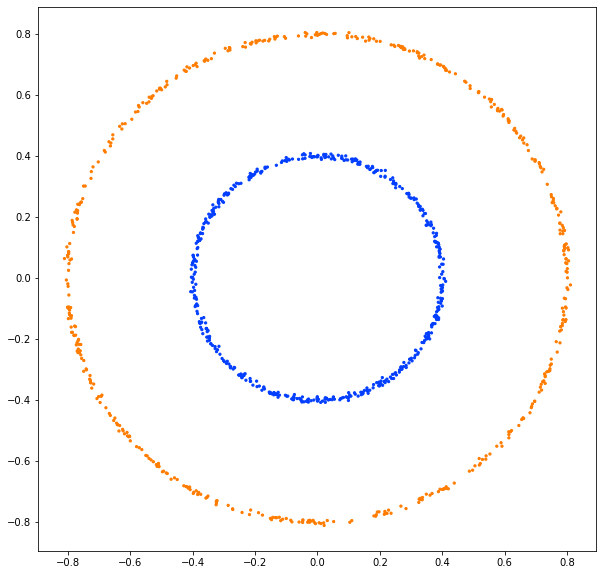
\includegraphics[width=0.49\linewidth]{figures/original_2_circles.png}}
    \subfigure[]{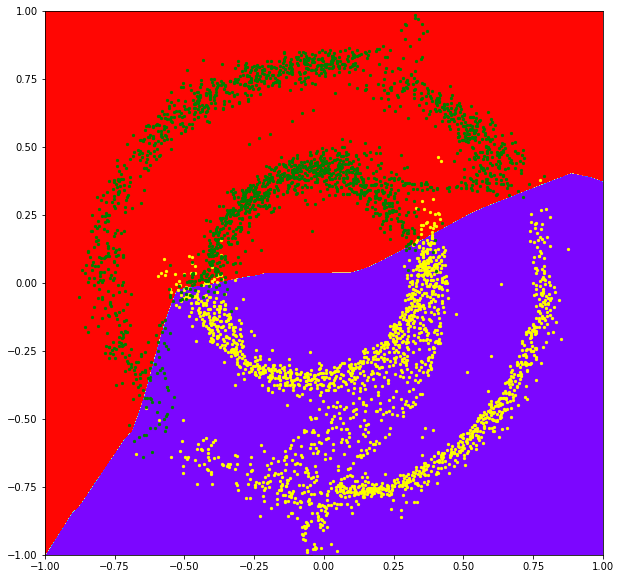
\includegraphics[width=0.49\linewidth]{figures/trained_2_circles_2.png}}
  \end{subfigmatrix}
    \caption{(a) Original dataset. (b) Samples from the learned model, without
    any labels. Coloring logic is the same as in \ref{fig:pinwheel}.}
\label{fig:twocircles}
\end{figure}

\begin{figure}[!htb]
  \begin{subfigmatrix}{2}
    \subfigure[]{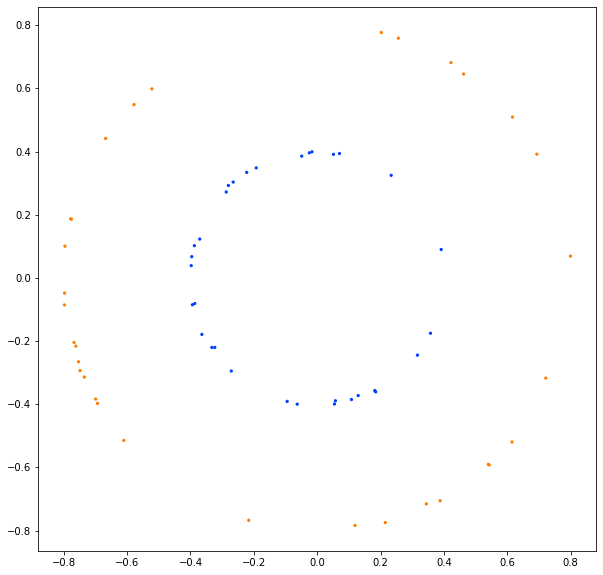
\includegraphics[width=0.49\linewidth]{figures/labeled_2_circles.png}}
    \subfigure[]{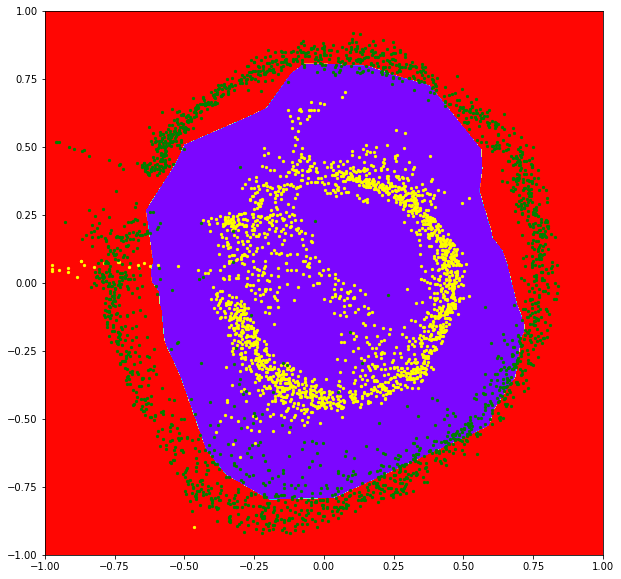
\includegraphics[width=0.49\linewidth]{figures/trained_2_circles_semisup.png}}
  \end{subfigmatrix}
    \caption{(a) Labeled points used in semi-supervised scenario. (b) Samples
    from the model trained in the semi-supervised scenario.}
\label{fig:twocircles-semisup}
\end{figure}

\subsection{Real-world dataset}
In this subsection, the proposed model is evaluated on the well-known MNIST
dataset \autocite{MNIST}. This dataset consists of images of handwritten digits.
The grids are of dimension 28 x 28 and were flattened to vectors of dimension 784
for training. For this experiment, only the images corresponding to the digits
from 0 to 4 were considered. The normalizing flow model used for the components
was a MAF, with 5 blocks, whose internal MADE layers had 1 hidden layer of dimension
200. The variational posterior was parameterized by a multi-layer perceptron, with
1 hidden layer of dimension 512. The model was trained for 100 epochs, with a mini-batch
size of 100. The Adam optimizer was used, with a learning rate of 0.0001, and with
a weight decay parameter of 0.000001. In Figure \ref{fig:mnist_samples}, samples
from the components obtained after training can be seen. Moreover, a normalized
contingency table is presented, where the performance of the variational posterior
as a clustering function can be assessed. Note that the cluster indices induced
by the model have no semantic meaning.

\begin{figure}[!htb]
  \centering
  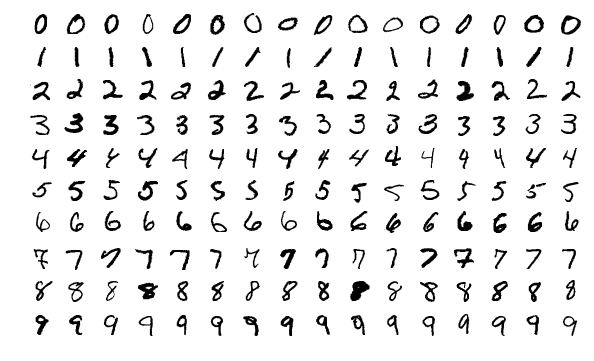
\includegraphics[width=0.85\linewidth]{figures/trained_mnist.png}
  \caption{Samples from the fitted mixture components. Each row is sampled
  from the same component}
  \label{fig:mnist_samples}
\end{figure}

\begin{table}[h]
\centering
\begin{tabular}{cccccc}
\toprule
\diagbox[trim=lr]{True\\label}{Cluster\\index} &         0 &         1 &         2 &         3 &         4 \\
\midrule
0    &  0.000602 &  0.012432 &  0.002807 &  0.982555 &  0.001604 \\
1    &  0.002139 &  0.020146 &  0.977001 &  0.000178 &  0.000535 \\
2    &  0.000802 &  0.952276 &  0.011630 &  0.007219 &  0.028073 \\
3    &  0.001558 &  0.479455 &  0.300682 &  0.004284 &  0.214021 \\
4    &  0.646166 &  0.347273 &  0.005125 &  0.001435 &  0.000000 \\
\bottomrule
\end{tabular}
\caption{Normalized contingency table for the clustering induced by the model}
\label{table:contingency}
\end{table}

From Table \ref{table:contingency} and Figure \ref{fig:mnist_samples} it is possible
to see that although there is some confusion, the model successfully clusters
the MNIST digits.
